\documentclass[12pt, a4paper, oneside]{amsart}
\setlength{\parindent}{0pt}
\usepackage[margin=2cm]{geometry}
\usepackage{amsmath}
\usepackage{amssymb}
\usepackage{amsfonts}
\usepackage[pdftex]{graphicx}
\usepackage[usenames]{color}
\usepackage{graphicx}
\usepackage{hyperref}
\usepackage{amsthm}

\title{Project 5: Text Manipulation on E-Mail Messages}
\author{Kevin Fujii and Erin Melcon}
\date{\today}

\begin{document}

\maketitle

\section{Project Overview}

In this assignment, we focus on manipulating text data into a desirable form and analyzing the structured data through the application of regular expressions.  We will be using two large data sets for this project.  The first data set is composed of all e-mails from Enron before the company folded.  The second contains the archive of the R-help mailing list from April 1998 to February 2011.  The data sets have several aspects in common, so we can use these characteristics to create general functions that should be compatible with all e-mail files.

\section{R-Help mailing list}

\subsection{Format of the data}

The R-help mailing list archive is stored as 167 .tar.gz files corresponding to each month from April 1998 to February 2011.  Each of the .tar.gz files is a compressed text file consisting of all e-mail messages send through the mailing list during that month.  

\subsection{Trend over time}

E-mail volume per month varies from 36 to 8674 messages, and there is an increasing trend through time.  A plot of the e-mail messages sent per month may be seen in Figure \ref{fig:rhelpByMonth}.

\begin{figure}[htp]
\centering
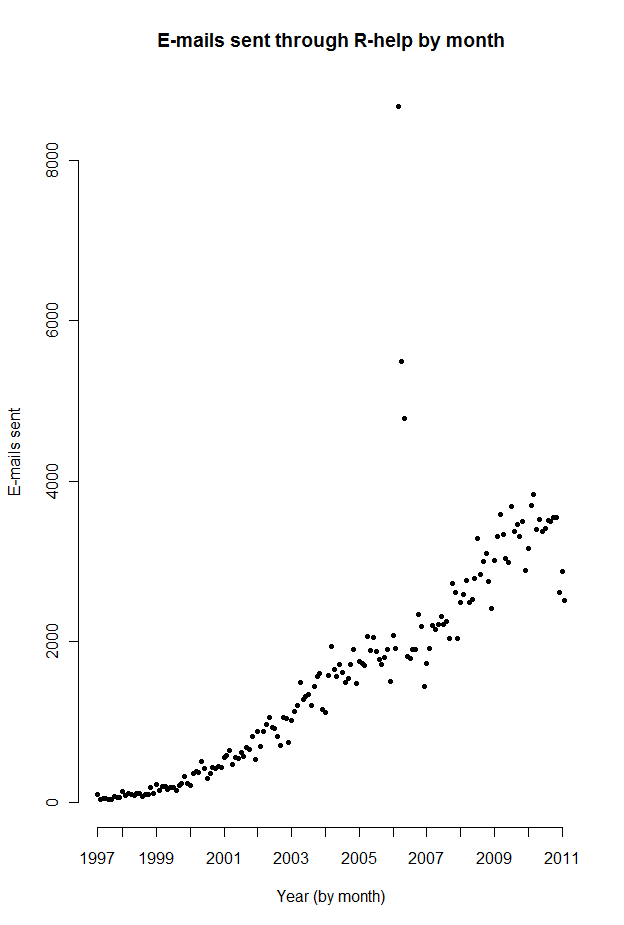
\includegraphics[width = 100mm]{rhelpByMonth.png}
\caption{From 1998 to 2011, the popularity of the R-help mailing list appears to grow exponentially with some unexpectedly high traffic during 2006.}\label{fig:rhelpByMonth}
\end{figure}

Upon closer inspection, the spike in e-mail volume seen in Figure \ref{fig:rhelpByMonth} occurs in March 2006.  As a diagnostic check, we can look at the file size corresponding to the compressed file of that month's e-mail messages, and sure enough, the March 2006 file is much larger than the other files.  We can take a closer look at e-mail volume by inspecting the data set by day rather than by month.  A histogram of e-mail volume by day is shown in Figure \ref{fig:rhelpByDay}.

\begin{figure}[htp]
\centering
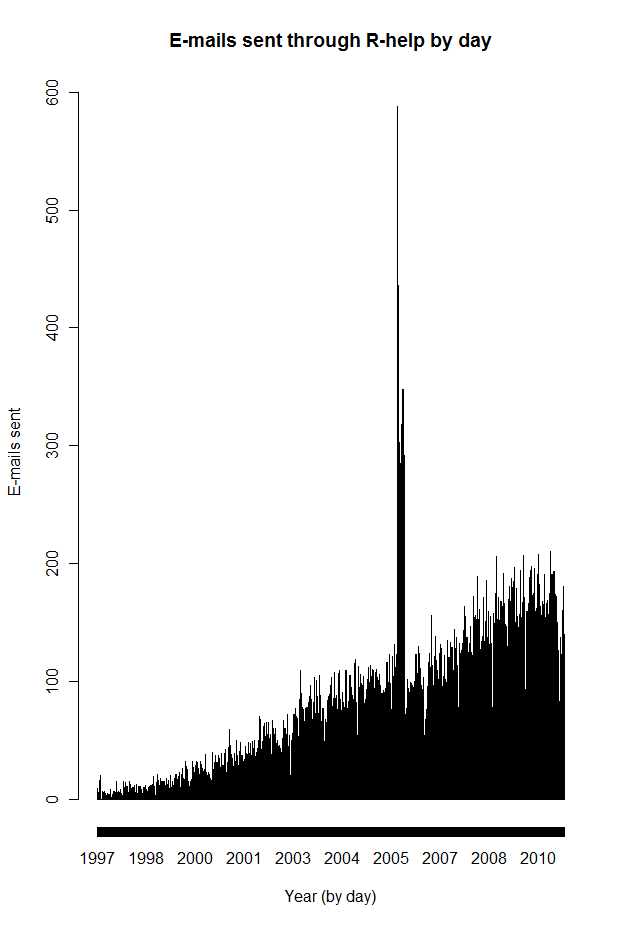
\includegraphics[width = 100mm]{rhelpByDay.png}
\caption{The e-mail volume appears to grow when we look at e-mails sent per day.  The peaks occur in March 2006, when around 500 e-mails were sent on multiple days.}\label{fig:rhelpByDay}
\end{figure}

Somewhat unsurprisingly at this point, the 49 days with the most e-mails sent through the R-help mailing list all occurred in 2006.  All of these 49 days fell in March, April, or May of that year.  Looking at a plot of the number of unique users per month, as in Figure \ref{fig:uniqueUsers}, we see that there are no clear outliers.  This is an indication that the number of e-mails sent in those few months in 2006 may have been artificially increased.  Upon closer inspection of the day with the heaviest traffic (March 6th, 2006), it appears that every person sent a multiple of four e-mails.  In fact, looking at the bodies of the e-mails, the messages sent on that day were replicated in the data set four times, which explains the high e-mail volume on that day.  Since Figure \ref{fig:rhelpByDay} shows that the e-mail volume was unexpectedly high on multiple days, we looked at all days in 2006 for the same pattern.  It appears that from March 1st through 17th, the messages were replicated four times for some reason.

\begin{figure}[htp]
\centering
\includegraphics[width = 100mm]{uniqueUsers.png}
\caption{The unique users of the R-help mailing list does not display any outliers, suggesting that the e-mail volume peaks in 2006 may be artificial.}\label{fig:uniqueUsers}
\end{figure}

Let's look at the dates by day of the week to see if any trends are apparent there.  A bar graph of e-mail frequency by day of the week is shown in Figure \ref{fig:weekdays}.  It appears that e-mail volume drops significantly on Saturdays and Sundays.  E-mails were most commonly sent in the middle of the week with slightly fewer e-mails sent on Mondays and Fridays.  It certainly makes sense that the e-mail volume was higher during weekdays; on those days, people are much more likely to be at work, and thus may request help as problems arise.

\begin{figure}[htp]
\centering
\includegraphics[width = 100mm]{weekdays.png}
\caption{E-mails were much more commonly sent in the middle of the week than during the weekends.}\label{fig:weekdays}
\end{figure}

Finally, let's see if our hypothesis about people using the R-help mailing list while at work (during working hours) is supported by the data itself.  Looking at the ``Date:'' field of the header, we can also extract the (local) time that each e-mail message was sent.  It's important to work with local times here because, as shown later, people using the mailing list use domains from around the world.  After extracting the times, we can make a bar graph of e-mails sent during each hour of the day, shown in Figure \ref{fig:hours}.  The graph shows a logical trend: E-mails to the R-help mailing list increase sharply around 8 or 9 in the morning, and decrease throughout the afternoon and night.  This seems to corroborate our hypothesis.  We also notice that, aside from a small decline in e-mail volume between 12 and 2 in the afternoon, the trend is fairly smooth otherwise.  This small deviation could be caused by people at work taking a lunch break, and thus they wouldn't be sending e-mails to the R-help mailing list.

\begin{figure}[htp]
\centering
\includegraphics[width = 100mm]{hours.png}
\caption{The trend of e-mails sent per hour seems consistent with a 9-to-5 work day.}\label{fig:hours}
\end{figure}

\subsection{Functions of interest}

We can use regular expressions in order to search the subjects and bodies of the R-help e-mails for function calls.  A proposed method for searching for function calls is to look for alphanumeric characters or periods immediately before a left open parenthesis.  This method should find all function calls (with proper syntax).  There may be some false positives allowed by this method, but this should be nearly inconsequential for our purposes.  We aim to figure out the most commonly used or asked-about functions in the R-help mailing list.  First, let's look through the subject lines.  A search with regular expressions found 19150 possible uses of functions in subject lines, the most common of which are tabulated in the first two columns of Table \ref{table:allFcns}.

 \begin{table}[ht]
 \centering
 \begin{tabular}{|c|c||c|c|}
 \hline
\multicolumn{2}{|c||}{Subject Line} & \multicolumn{2}{|c|}{E-Mail Body}\\
\hline
\footnotesize{\textbf{Function}}& \footnotesize{\textbf{Frequency}} & \footnotesize{\textbf{Function}}& \footnotesize{\textbf{Frequency}}\\
\hline
lm & 527 & c & 169356 \\
plot & 465 & function & 55049\\
par & 326 & list & 39738\\
library & 242 & library & 31071\\
apply & 213 & plot & 30538\\
optim & 194 & length & 29409\\
glm & 191 & rep & 28783\\
source & 191 & rnorm & 24379\\
c & 183 & data.frame & 22974\\
summary & 181 & paste & 21357\\
lme & 178 & matrix & 20023\\
image & 166 & lm & 16186\\
\hline
\end{tabular}
\caption{The twelve most commonly referenced functions in subject lines and e-mail bodies from the R-help mailing list.}
\label{table:allFcns}
\end{table}

The functions appearing in Table \ref{table:allFcns} are all quite common, as expected.  Several of them (also including \textit{lmer}, not listed in Table \ref{table:allFcns}) refer to various types of linear models, indicating that many people are using the R-help mailing list for advice or troubleshooting when performing data analysis.  Further, graphical and summarizing functions appear on the list, which are used to visually or numerically summarize a data set.

Now, let's look at the functions used in the bodies of the e-mail messages.  The most commonly used functions in e-mail bodies are displayed in the third and fourth columns of Table \ref{table:allFcns}.  It should come as no surprise that the functions used in e-mail bodies are even more generic than those in subject lines.  Users of the R-help mailing list are likely to include their code in the bodies of their e-mails, so it makes sense that these generic functions appear most often since they have wide applications.  Many of these functions deal with data creation, possibly to set up test data for more complex function calls.

We can also explore what packages the users of the R-help mailing list are utilizing.  The most commonly loaded packages are shown in Table \ref{table:allLibs}.

 \begin{table}[ht]
 \centering
 \begin{tabular}{|c|c||c|c|}
 \hline
\multicolumn{2}{|c||}{Subject Line} & \multicolumn{2}{|c|}{E-Mail Body}\\
\hline
\footnotesize{\textbf{Library}}& \footnotesize{\textbf{Frequency}} & \footnotesize{\textbf{Library}}& \footnotesize{\textbf{Frequency}}\\
\hline
survival & 13 & lattice & 2392 \\
car &10 & zoo & 1384\\
MASS & 10 & MASS & 1345\\
gplots & 9 & nlme & 1005\\
Matrix & 9 & ggplot2 & 824\\
... & 8 & Hmisc & 604\\
tcltk & 8 & chron & 555\\
fCalendar & 6 & lme4 & 497\\
SSPA & 6 & tcltk & 477\\
``package'' & 5 & RODBC & 471\\
svIDE & 5 & gsubfn & 393\\
convert & 4 & survival & 375\\
\hline
\end{tabular}
\caption{The twelve most commonly referenced libraries in subject lines and e-mail bodies from the R-help mailing list.}
\label{table:allLibs}
\end{table} 

\subsection{E-mail domains}

Let's take a look at the most common e-mail domains.  To do this, we must identify the headers of each e-mail, find the lines beginning with ``From:'', and extract the domain names from these lines.  After doing this for every e-mail header, we can tabulate the most common domains, shown in Table \ref{table:domains}.  In the same table, we also display the most active e-mail senders.

 \begin{table}[ht]
 \centering
 \begin{tabular}{|c|c||c|c|}
 \hline
\multicolumn{2}{|c||}{Most Common Domains} & \multicolumn{2}{|c|}{Most Active Senders}\\
\hline
\footnotesize{\textbf{Domain}}& \footnotesize{\textbf{Frequency}} & \footnotesize{\textbf{Sender}}& \footnotesize{\textbf{Frequency}}\\
\hline
gmail.com & 56288 & Prof Brian Ripley & 8959 \\
stats.ox.ac.uk &11490 & Gabor Grothendieck & 7942\\
yahoo.com & 8545 & Uwe Ligges & 5184\\
comcast.net & 5878 & David Winsemius & 4846\\
biostat.ku.dk & 5245 & Duncan Murdoch & 4500\\
hotmail.com & 4982 & Peter Dalgaard & 3300\\
statistik.uni-dortmund.de & 3619 & jim holtman & 3199\\
stats.uwo.ca & 3491 & Thomas Lumley & 2905\\
pdf.com & 2957 & Liaw, Andy & 2445\\
u.washington.edu & 2928 & Spencer Graves & 2413\\
merck.com & 2816 & Marc Schwartz & 2391\\
stat.math.ethz.ch & 2176 & Peter Dalgaard BSA & 2137\\
\hline
\end{tabular}
\caption{The twelve most commonly used e-mail domains and the twelve most active R-help e-mail senders.}
\label{table:domains}
\end{table} 

By comparing these tables, we can see that some of the most active senders account for the vast majority of e-mails sent to the R-help mailing list from their domain.  For example, Brian Ripley (ripley at stats.ox.ac.uk) sends nearly 78\% of the e-mails from the stats.ox.ac.uk domain.  Uwe Ligges sent e-mails through two domain names (statistik.tu-dortmund.de and statistik.uni-dortmund.de), and thus he ended up sending more e-mails than there were in total from his primary domain.  Not only did Peter Dalgaard have two forms of his name listed (Peter Dalgaard and Peter Dalgaard BSA), but he sent messages from several domains, including gmail.com, biostat.ku.dk, pubhealth.ku.dk, and cbs.dk.

\subsection{Message threads}

A more difficult task is to try to figure out which e-mails were in reply to others and to attempt to find the message threads in the mailing list.  Due to time constraints, we only looked at one level of e-mail replies among the first 20000 e-mails.  We created a list of all messages in this set that were not replies to any other e-mail.  Then, for each of these e-mails, we found the messages in the remaining set that were replies to it.  It turned out that one of the e-mails, sent by Indrajit SenGupta on April 2nd, 2002, was replied to 16 times.  The text of his e-mail is as follows:

\begin{quote}
Can we expect to see an R package on Statistical Quality Control in the      
future like SPLUS? I can't understand why nobody made this package before.    
                                                                             
                                                       
Indrajit SenGupta     
                                                        
Department Of Statistics   
                                                  
St. Xavier's College   
                                                        
Calcutta University  
                                                          
indra\_calisto at yahoo.com   
                                                  
indrajitsg at vsnl.net   
                                                                                                                                   
\end{quote}

It appears that this request drew some interest or suggestions from the readers of the mailing list, as this was the most popular e-mail to reply to among the first 20000 e-mails sent to the mailing list.

\newpage
\section{Enron Email List}
The main purpose of this part of the project is to find all the email recipients and senders from the Enron data set, and summarize and graphically represent the results.  The first task was to extract the header of the emails, and from this extract all of the information about who sent the email, and who it was sent to.  This included looking for Bcc (Blind Carbon Copy) and Cc (Carbon Copy) fields.\\
This was accomplished using regular expressions, and we found that if we do not include Bcc and Cc, we see that the person who emailed anyone the most was Jeff Dasovich.  If we include Bcc and Ccs, the list remains the same.  We may now want to investigate who Jeff was emailing, and we have two ways of doing that.\\ 
\begin{table}[h]
\begin{center}
\begin{tabular}{|r|l|r|}
  \hline
Rank & Sender & Number of Emails \\ 
  \hline
1 & jeff.dasovich@enron.com & 131302 \\ 
2 & veronica.espinoza@enron.com & 110601 \\ 
3 & rhonda.denton@enron.com & 90730 \\ 
4 & cheryl.johnson@enron.com & 74632 \\ 
5 & jae.black@enron.com & 59196 \\ 
 \hline
\end{tabular}
\caption{The top 5 people who sent email from the Enron email list.}
\label{table:allLibs}
\end{center}
\end{table}

The first is to build another frequency table, as follows:
\begin{table}[h]
\begin{center}
\begin{tabular}{|r|l|l|l|}
  \hline
Rank & Sender & Recipient & Frequency \\ 
  \hline
 1 & jeff.dasovich@enron.com & richard.shapiro@enron.com & 2909 \\ 
  2 & jeff.dasovich@enron.com & paul.kaufman@enron.com & 2768 \\ 
  3 & jeff.dasovich@enron.com & susan.mara@enron.com & 2746 \\ 
  4 & jeff.dasovich@enron.com & james.steffes@enron.com & 2725 \\ 
  5 & jeff.dasovich@enron.com & karen.denne@enron.com & 2489 \\ 
   \hline
\end{tabular}
\caption{The top five people that Jeff Dasovich emailed.}
\label{table:allLibs}
\end{center}
\end{table}
In which we can see the number of times Jeff emailed his top 5 recipients.  We may also look at a network graph;
\begin{figure}[htp]
\centering
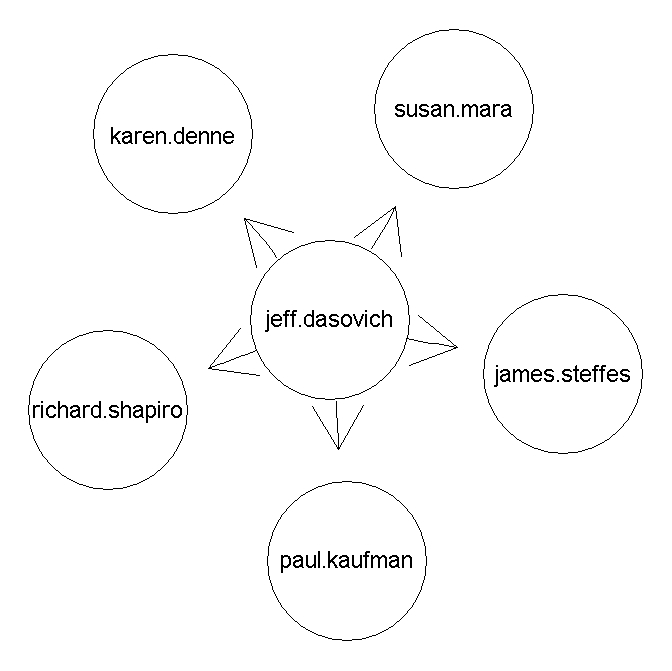
\includegraphics[width = 100mm]{JeffPlot.jpeg}
\caption{A small network of who Jeff emails}\label{fig:JeffNetwork}
\end{figure}\\
Which gives us the same information, but visually, and without information about the weights.  However, with network graphs it is easy to see who people Jeff emailed were communicating with.  
\begin{figure}[htp]
\centering
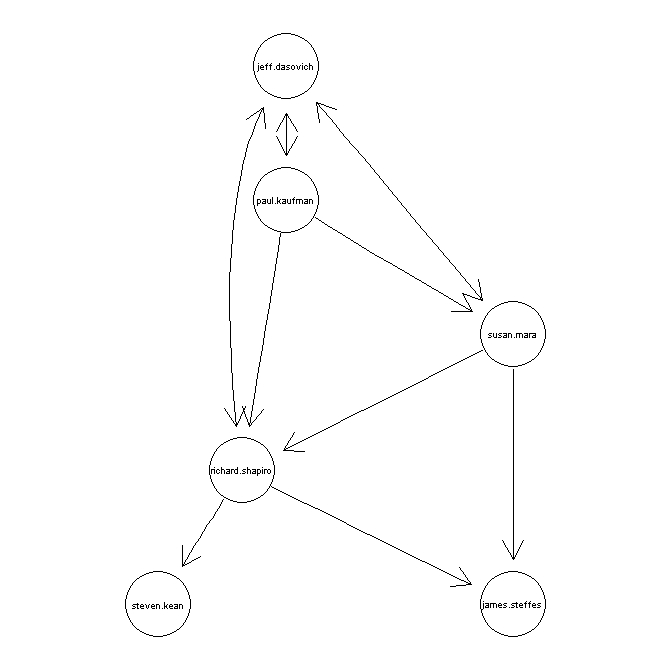
\includegraphics[width = 100mm]{JeffPlot2.jpeg}
\caption{A small network of who Jeff emails, and who they email.}\label{fig:JeffNetwork}
\end{figure}\\
This shows that there is a small group, some of which email each other frequently. 


\end{document}